\documentclass[11pt,a4paper]{report}
\usepackage[textwidth=37em,vmargin=30mm]{geometry}
\usepackage{calc,xunicode,amsmath,amssymb,paralist,enumitem,tabu,booktabs,datetime2,xeCJK,xeCJKfntef,listings}
\usepackage{tocloft,fancyhdr,tcolorbox,xcolor,graphicx,eso-pic,xltxtra,xelatexemoji}

\newcommand{\envyear}[0]{2024}
\newcommand{\envdatestr}[0]{2024-12-08}
\newcommand{\envfinaldir}[0]{webdb/2024/20241208/final}

\usepackage[hidelinks]{hyperref}
\hypersetup{
    colorlinks=false,
    pdfpagemode=FullScreen,
    pdftitle={Web Digest - \envdatestr}
}

\setlength{\cftbeforechapskip}{10pt}
\renewcommand{\cftchapfont}{\rmfamily\bfseries\large\raggedright}
\setlength{\cftbeforesecskip}{2pt}
\renewcommand{\cftsecfont}{\sffamily\small\raggedright}

\setdefaultleftmargin{2em}{2em}{1em}{1em}{1em}{1em}

\usepackage{xeCJK,xeCJKfntef}
\xeCJKsetup{PunctStyle=plain,RubberPunctSkip=false,CJKglue=\strut\hskip 0pt plus 0.1em minus 0.05em,CJKecglue=\strut\hskip 0.22em plus 0.2em}
\XeTeXlinebreaklocale "zh"
\XeTeXlinebreakskip = 0pt


\setmainfont{Brygada 1918}
\setromanfont{Brygada 1918}
\setsansfont{IBM Plex Sans}
\setmonofont{JetBrains Mono NL}
\setCJKmainfont{Noto Serif CJK SC}
\setCJKromanfont{Noto Serif CJK SC}
\setCJKsansfont{Noto Sans CJK SC}
\setCJKmonofont{Noto Sans CJK SC}

\setlength{\parindent}{0pt}
\setlength{\parskip}{8pt}
\linespread{1.15}

\lstset{
	basicstyle=\ttfamily\footnotesize,
	numbersep=5pt,
	backgroundcolor=\color{black!5},
	showspaces=false,
	showstringspaces=false,
	showtabs=false,
	tabsize=2,
	captionpos=b,
	breaklines=true,
	breakatwhitespace=true,
	breakautoindent=true,
	linewidth=\textwidth
}






\newcommand{\coverpic}[2]{
    % argv: itemurl, authorname
    Cover photo by #2~~(\href{#1}{#1})
}
\newcommand{\makeheader}[0]{
    \begin{titlepage}
        % \newgeometry{hmargin=15mm,tmargin=21mm,bmargin=12mm}
        \begin{center}
            
            \rmfamily\scshape
            \fontspec{BaskervilleF}
            \fontspec{Old Standard}
            \fontsize{59pt}{70pt}\selectfont
            WEB\hfill DIGEST
            
            \vfill
            % \vskip 30pt
            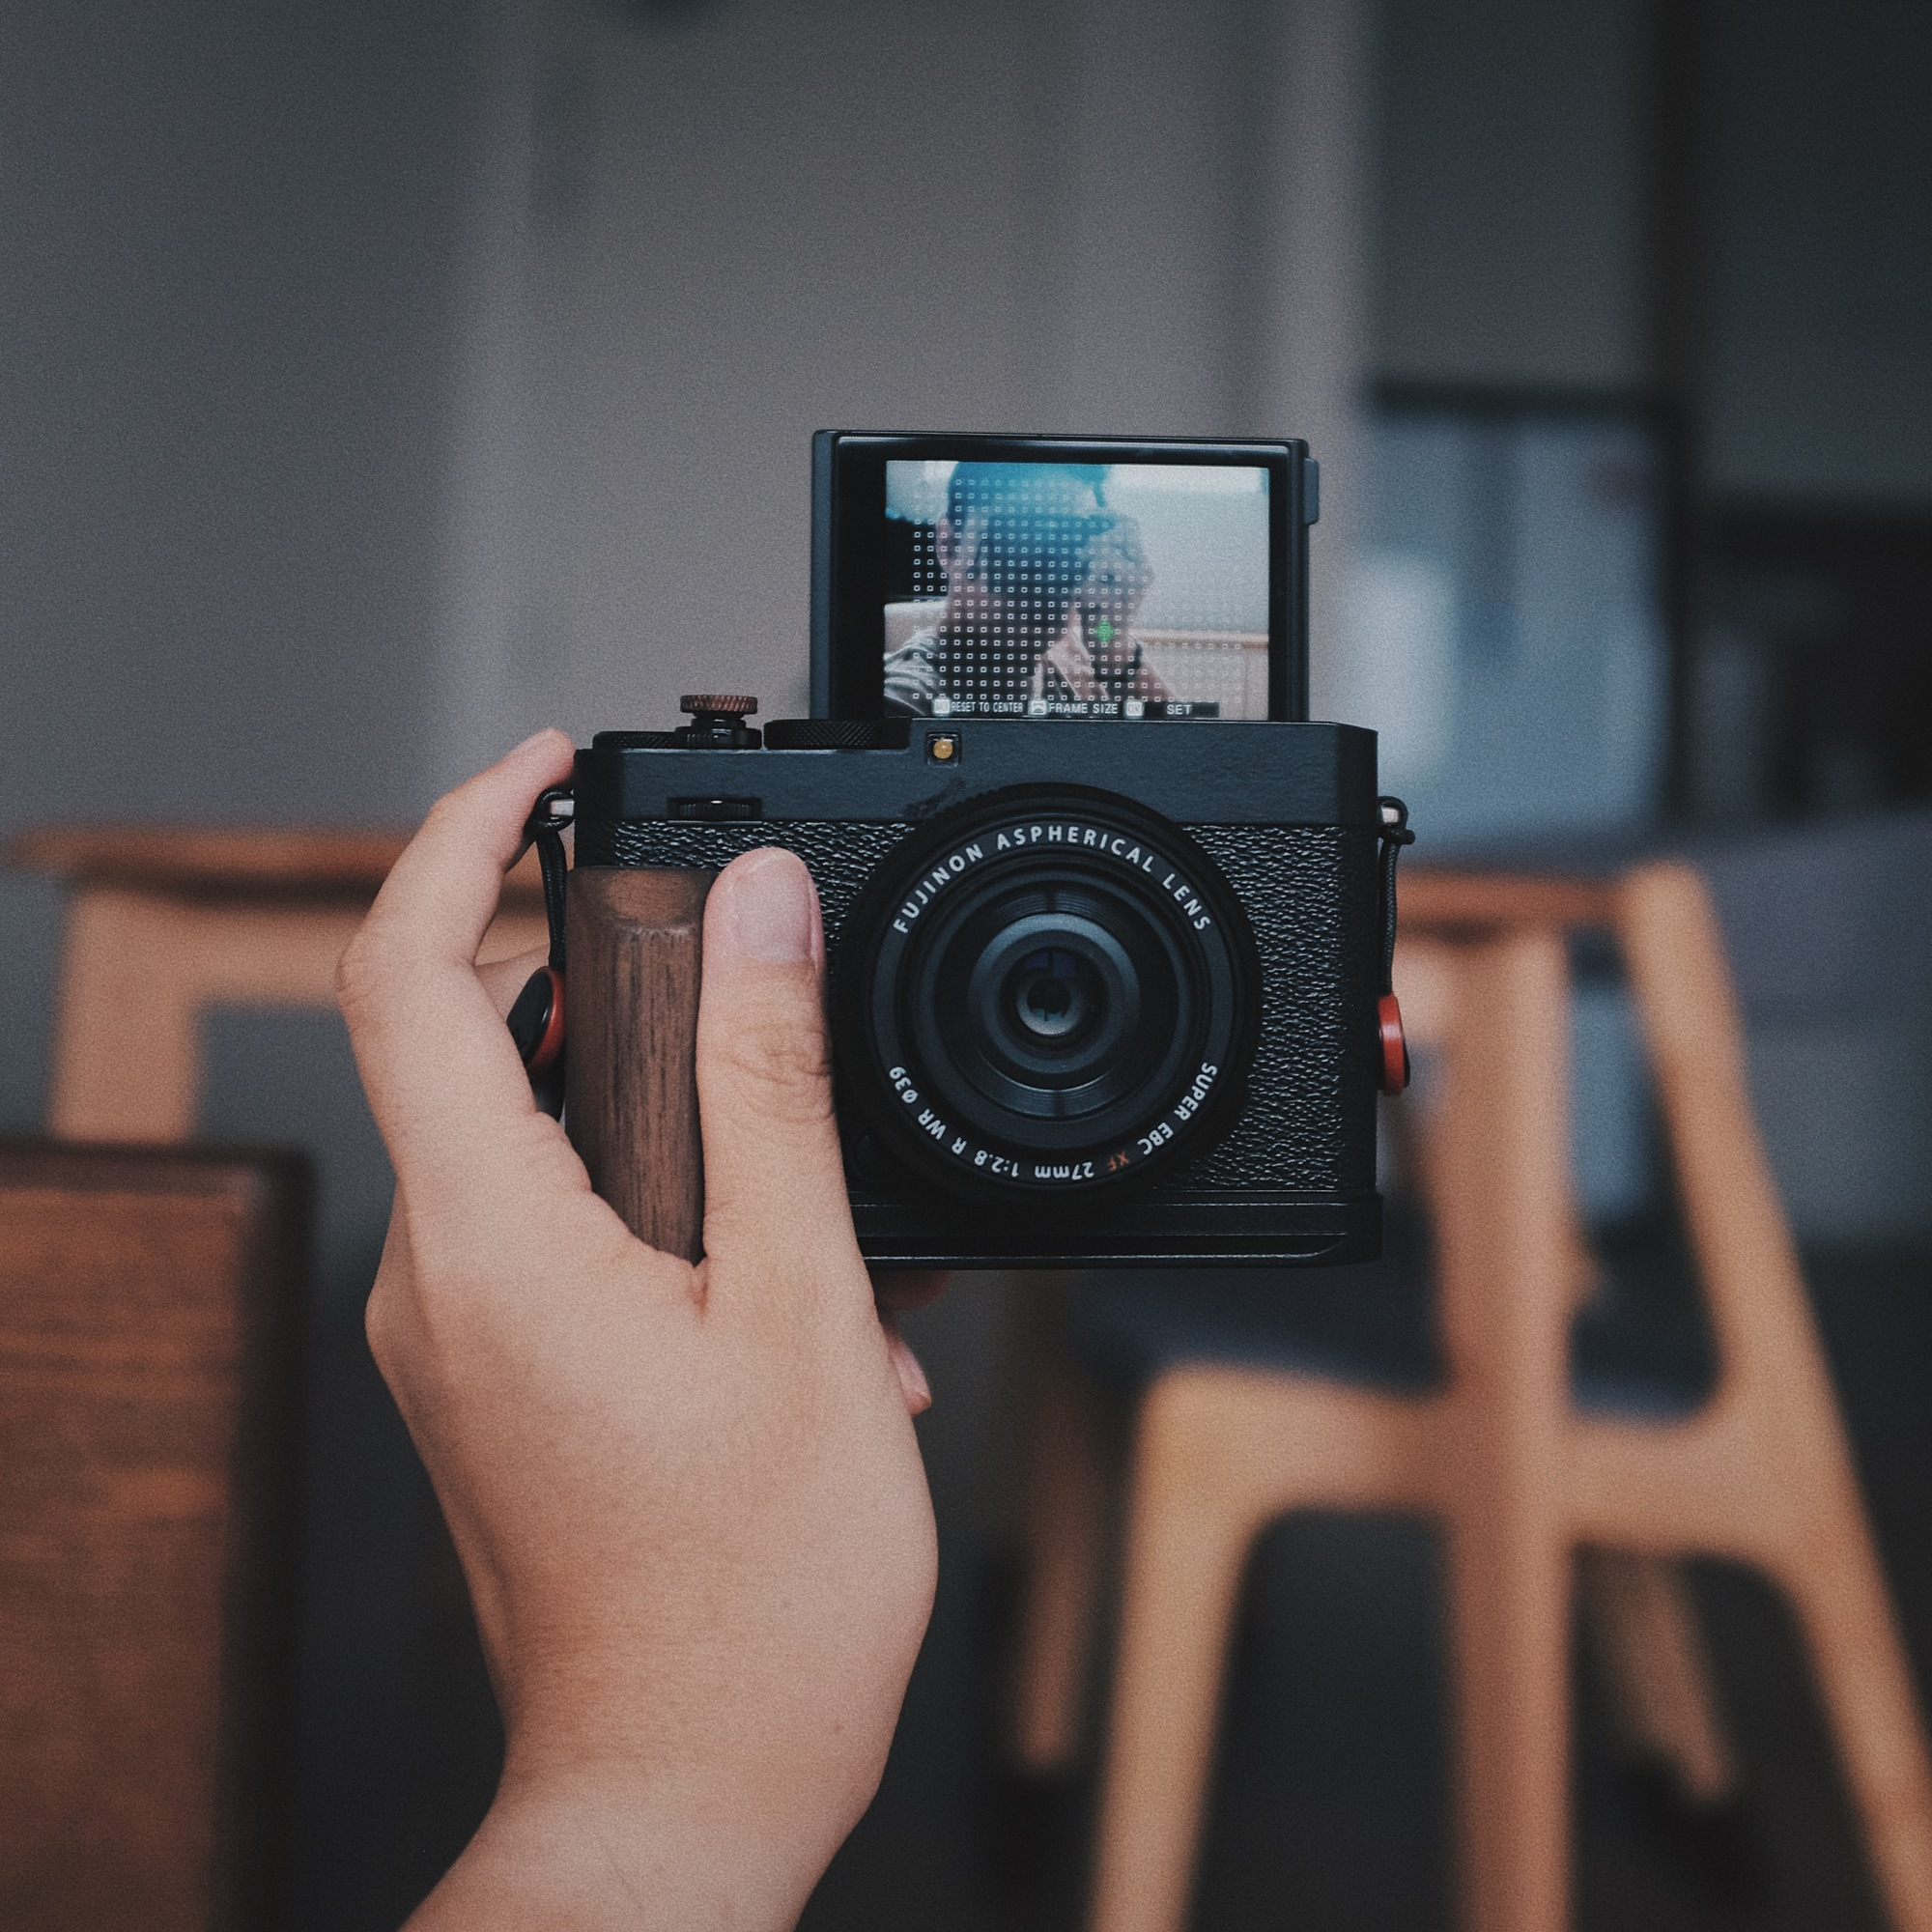
\includegraphics[width=\linewidth]{\envfinaldir/coverpic-prod.jpg}\par
            % \vskip 30pt
            \vfill

            \normalsize\rmfamily\scshape
            \copyright{} The Web Digest Project \hfill\large \envdatestr
        \end{center}
    \end{titlepage}
    % \restoregeometry
}
\newcommand{\simplehref}[1]{%
    \textcolor{blue!80!green}{\href{#1}{#1}}%
}
\renewcommand{\contentsname}{\center\Huge\sffamily\bfseries Contents\par\vskip 20pt}
\newcounter{ipartcounter}
\setcounter{ipartcounter}{0}
\newcommand{\ipart}[1]{
    % \vskip 20pt
    \clearpage
    \stepcounter{ipartcounter}
    \phantomsection
    \addcontentsline{toc}{chapter}{#1}
    % \begin{center}
    %     \Huge
    %     \sffamily\bfseries
    %     #1
    % \end{center}
    % \vskip 20pt plus 7pt
}
\newcounter{ichaptercounter}
\setcounter{ichaptercounter}{0}
\newcommand{\ichapter}[1]{
    % \vskip 20pt
    \clearpage
    \stepcounter{ichaptercounter}
    \phantomsection
    \addcontentsline{toc}{section}{\numberline{\arabic{ichaptercounter}}#1}
    \begin{center}
        \Huge
        \sffamily\bfseries
        #1
    \end{center}
    \vskip 20pt plus 7pt
}
\newcommand{\entrytitlefont}[1]{\subsection*{\raggedright\Large\sffamily\bfseries#1}}
\newcommand{\entryitemGeneric}[2]{
    % argv: title, url
    \parbox{\linewidth}{
        \entrytitlefont{#1}\par\vskip 5pt
        \footnotesize\ttfamily\mdseries
        \simplehref{#2}
    }\vskip 11pt plus 11pt minus 1pt
}
\newcommand{\entryitemGithub}[3]{
    % argv: title, url, desc
    \parbox{\linewidth}{
        \entrytitlefont{#1}\par\vskip 5pt
        \footnotesize\ttfamily\mdseries
        \simplehref{#2}\par\vskip 5pt
        \small\rmfamily\mdseries#3
    }\vskip 11pt plus 11pt minus 1pt
}
\newcommand{\entryitemAp}[3]{
    % argv: title, url, desc
    \parbox{\linewidth}{
        \entrytitlefont{#1}\par\vskip 5pt
        \footnotesize\ttfamily\mdseries
        \simplehref{#2}\par\vskip 5pt
        \small\rmfamily\mdseries#3
    }\vskip 11pt plus 11pt minus 1pt
}
\newcommand{\entryitemHackernews}[3]{
    % argv: title, hnurl, rawurl
    % \parbox{\linewidth}{
    %     \entrytitlefont{#1}\par\vskip 5pt
    %     \footnotesize\ttfamily\mdseries
    %     \simplehref{#3}\par
    %     \textcolor{black!50}{\href{#2}{#2}}
    % }\vskip 11pt plus 11pt minus 1pt
    \begin{minipage}{\linewidth}
            \entrytitlefont{#1}\par\vskip 5pt
            \footnotesize\ttfamily\mdseries
            \simplehref{#3}\par
            \textcolor{black!50}{\href{#2}{#2}}
    \end{minipage}\par\vskip 11pt plus 11pt minus 1pt
}







\begin{document}

\makeheader

\tableofcontents\clearpage




\ipart{Developers}
\ichapter{Hacker News}
\entryitemTwoLinks{Airline informant received thousands from passenger cash seizures}{https://news.ycombinator.com/item?id=42354580}{https://www.atlantanewsfirst.com/2024/12/03/airline-informant-received-thousands-passenger-cash-seizures/}

\entryitemTwoLinks{Browsing negative content online makes mental health struggles worse: Study}{https://news.ycombinator.com/item?id=42353944}{https://news.mit.edu/2024/study-browsing-negative-content-online-makes-mental-health-struggles-worse-1205}

\entryitemTwoLinks{Notre Dame Cathedral reopens}{https://news.ycombinator.com/item?id=42353215}{https://apnews.com/article/notre-dame-paris-latest-e50813cf016f08607c20ab115bc4b153}

\entryitemTwoLinks{Raspberry Pi 5 now supports Valve's Steam Link}{https://news.ycombinator.com/item?id=42352371}{https://www.raspberrypi.com/news/valves-steam-link-on-raspberry-pi/}

\entryitemTwoLinks{Just: Just a Command Runner}{https://news.ycombinator.com/item?id=42351101}{https://just.systems/}

\entryitemTwoLinks{Protecting undersea internet cables is a tech nightmare}{https://news.ycombinator.com/item?id=42350584}{https://spectrum.ieee.org/undersea-internet-cables-protection-tech}

\entryitemTwoLinks{Tell HN: Need help, locked out of Google account with 10 years of personal data}{https://news.ycombinator.com/item?id=42350245}{https://news.ycombinator.com/item?id=42350245}

\entryitemTwoLinks{Police illegally sell restricted weapons, supplying crime}{https://news.ycombinator.com/item?id=42349858}{https://www.cbsnews.com/news/police-selling-restricted-guns-posties/}

\entryitemTwoLinks{Mathics 7.0 – Open-source alternative to Mathematica}{https://news.ycombinator.com/item?id=42349375}{https://github.com/Mathics3/mathics-core/releases/tag/7.0.0}

\entryitemTwoLinks{Show HN: Countless.dev – A website to compare every AI model: LLMs, TTSs, STTs}{https://news.ycombinator.com/item?id=42348513}{https://countless.dev/}

\entryitemTwoLinks{An invisible desktop application that will help you pass technical interviews}{https://news.ycombinator.com/item?id=42348147}{https://github.com/ibttf/interview-coder}

\entryitemTwoLinks{Can life emerge around a white dwarf?}{https://news.ycombinator.com/item?id=42348085}{https://www.centauri-dreams.org/2024/12/06/can-life-emerge-around-a-white-dwarf/}

\entryitemTwoLinks{How to use Postgres for everything}{https://news.ycombinator.com/item?id=42347606}{https://github.com/Olshansk/postgres\_for\_everything}

\entryitemTwoLinks{RollerCoaster Tycoon was the last of its kind [video]}{https://news.ycombinator.com/item?id=42346463}{https://www.youtube.com/watch?v=0JouTsMQsEA}

\entryitemTwoLinks{Structured Outputs with Ollama}{https://news.ycombinator.com/item?id=42346344}{https://ollama.com/blog/structured-outputs}

\entryitemTwoLinks{Biggest shell programs}{https://news.ycombinator.com/item?id=42346274}{https://github.com/oils-for-unix/oils/wiki/The-Biggest-Shell-Programs-in-the-World}

\entryitemTwoLinks{OpenWrt One router officially launched}{https://news.ycombinator.com/item?id=42345500}{https://openwrt.org/\#openwrt\_one\_router\_officially\_launched}

\entryitemTwoLinks{My second year without a job}{https://news.ycombinator.com/item?id=42344002}{https://shilin.ca/my-second-year-without-job/}

\entryitemTwoLinks{Lies I was told about collab editing, Part 1: Algorithms for offline editing}{https://news.ycombinator.com/item?id=42343953}{https://www.moment.dev/blog/lies-i-was-told-pt-1}

\entryitemTwoLinks{Does Your Code Pass the Turkey Test? (2008)}{https://news.ycombinator.com/item?id=42343920}{http://www.moserware.com/2008/02/does-your-code-pass-turkey-test.html}\ichapter{Phoronix}
\entryitemGeneric{\hskip 0pt{}More Kernel Bitrot: Old \& Busted UltraSPARC T2 "Niagara 2" SPU Driver Slated For Removal}{https://www.phoronix.com/news/Niagara-2-SPU-Driver-Bitrot}

\entryitemGeneric{\hskip 0pt{}OpenWrt Affected By Security Issue That Could Have Led To Compromised Build Artifacts}{https://www.phoronix.com/news/OpenWrt-Compromised-ASU-Builds}

\entryitemGeneric{\hskip 0pt{}UMD Direct Submission "Proof Of Concept" For The Intel Xe Linux Driver}{https://www.phoronix.com/news/UMD-Direct-Submit-Intel-Xe}

\entryitemGeneric{\hskip 0pt{}AMD Hardware Feedback Interface "HFI" Patches Updated For The Linux Kernel}{https://www.phoronix.com/news/AMD-HFI-v7-Linux}

\entryitemGeneric{\hskip 0pt{}Microsoft's Azure Linux 3.0 Adds 64K Kernel Option, NFTables \& Intel E800 Networking}{https://www.phoronix.com/news/Azure-Linux-3.0.20241203}

\entryitemGeneric{\hskip 0pt{}KDE Starts December By Landing A Number Of New Features}{https://www.phoronix.com/news/KDE-New-Features-December-2024}

\entryitemGeneric{\hskip 0pt{}OBS Studio 31.0 Released With New Features For Screen Recording \& Screencasting}{https://www.phoronix.com/news/OBS-Studio-31.0}

\entryitemGeneric{\hskip 0pt{}Wine 10.0-rc1 Released With Updated VKD3D, Initial Bluetooth Driver}{https://www.phoronix.com/news/Wine-10.0-rc1-Released}

\entryitemGeneric{\hskip 0pt{}Linux 6.13 Features: AutoFDO+Propeller Optimizations, Many AMD Additions \& SDUC + NVMe 2.1 Support}{https://www.phoronix.com/review/linux-613-features}


\ipart{Developers~~~~(zh-Hans)}
\ichapter{Solidot}
\entryitemGeneric{\hskip 0pt{}苹果引入百度 AI 面临诸多挑战}{https://www.solidot.org/story?sid=79984}

\entryitemGeneric{\hskip 0pt{}美国上诉法院维持 TikTok 强制出售法案 }{https://www.solidot.org/story?sid=79983}

\entryitemGeneric{\hskip 0pt{}为提高生育率东京政府为公务员提供四天工作制}{https://www.solidot.org/story?sid=79982}

\entryitemGeneric{\hskip 0pt{}罗马尼亚宪法法院宣布首轮总统大选无效}{https://www.solidot.org/story?sid=79981}

\entryitemGeneric{\hskip 0pt{}普通用户手机上发现间谍软件 Pegasus}{https://www.solidot.org/story?sid=79980}

\entryitemGeneric{\hskip 0pt{}教宗有了改装过的奔驰教宗纯电汽车}{https://www.solidot.org/story?sid=79979}

\entryitemGeneric{\hskip 0pt{}非人类动物没有发现不公平厌恶的证据}{https://www.solidot.org/story?sid=79978}

\entryitemGeneric{\hskip 0pt{}Linux 6.12 被选为最新的长期支持内核}{https://www.solidot.org/story?sid=79977}

\entryitemGeneric{\hskip 0pt{}古巴再次遭遇大规模断电}{https://www.solidot.org/story?sid=79976}

\entryitemGeneric{\hskip 0pt{}小米电动汽车季度销量超过丰田}{https://www.solidot.org/story?sid=79975}

\entryitemGeneric{\hskip 0pt{}气温升高加剧物种灭绝风险}{https://www.solidot.org/story?sid=79974}

\entryitemGeneric{\hskip 0pt{}GitLab 任命 Bill Staple 为新 CEO}{https://www.solidot.org/story?sid=79973}

\entryitemGeneric{\hskip 0pt{}OpenAI 推出 200 美元月费的 ChatGPT Pro}{https://www.solidot.org/story?sid=79972}

\entryitemGeneric{\hskip 0pt{}人人影视公开了其全部字幕存档}{https://www.solidot.org/story?sid=79971}

\entryitemGeneric{\hskip 0pt{}HowStuffWorks 创始人自杀身亡}{https://www.solidot.org/story?sid=79970}

\entryitemGeneric{\hskip 0pt{}黑客通过供应链攻击窃取了 15.5 万美元加密货币}{https://www.solidot.org/story?sid=79969}

\entryitemGeneric{\hskip 0pt{}短时间剧烈运动能显著降低女性的心血管疾病风险}{https://www.solidot.org/story?sid=79968}

\entryitemGeneric{\hskip 0pt{}明年全球云计算投资将 1.5 倍于阿波罗计划}{https://www.solidot.org/story?sid=79967}

\entryitemGeneric{\hskip 0pt{}Google DeepMind 称其天气预报模型 GenCast 比传统方法更准确}{https://www.solidot.org/story?sid=79966}

\entryitemGeneric{\hskip 0pt{}Windows 11 份额增长停滞}{https://www.solidot.org/story?sid=79965}


\ipart{Generic News}
\ichapter{AP News}
\entryitemWithDescription{\hskip 0pt{}Stolen ruby slippers worn by Judy Garland in `The Wizard of Oz' are auctioned for \$28 million}{https://apnews.com/article/6d5ccf8af71e1d7941d6f01ae4653b76}{}

\entryitemWithDescription{\hskip 0pt{}Far-right influencer Nick Fuentes accused of pepper spraying woman on his doorstep}{https://apnews.com/article/25e77dc172c2612ae24ba41c9fb45f89}{}

\entryitemWithDescription{\hskip 0pt{}Florida prosecutor seeks to clear records of people charged with buying police-made crack in 1980s}{https://apnews.com/article/796f5572af1757e368ae7a359e34bbae}{}

\entryitemWithDescription{\hskip 0pt{}Storm Darragh batters UK and Ireland, leaving 1 dead and hundreds of thousands without power}{https://apnews.com/article/f9d74be4f3516eea499033aaf0f4f0d1}{}

\entryitemWithDescription{\hskip 0pt{}Shesterkin's deal with the Rangers makes him the highest-paid goaltender in NHL history, reports say}{https://apnews.com/article/83f1307b994bea9ce6d751fb39e0170f}{}

\entryitemWithDescription{\hskip 0pt{}Mother of Austin Tice, journalist missing in Syria, says new information proves her son is alive}{https://apnews.com/article/58e79b5bcb117cac5674b27ff66d5d69}{}

\entryitemWithDescription{\hskip 0pt{}Pitcher Clay Holmes agrees to \$38 million, 3-year contract with Mets, AP source says}{https://apnews.com/article/f88434a752b9ba7e80f4052792a92268}{}

\entryitemWithDescription{\hskip 0pt{}Jury awards \$310 million to parents of teen killed in fall from Orlando amusement park ride}{https://apnews.com/article/899b45fcf4ee74bce47d6326727716cd}{}

\entryitemWithDescription{\hskip 0pt{}Princess of Wales takes another step in return to public life after chemotherapy with carol service}{https://apnews.com/article/fb2d9330ac9da508afbd2064d30440b5}{}

\entryitemWithDescription{\hskip 0pt{}Hall of Famer Randy Moss is stepping away from ESPN for an extended time to deal with health issue}{https://apnews.com/article/6e17260729b0ae89034db0d081981e82}{}

\entryitemWithDescription{\hskip 0pt{}More than a million oven gloves are being recalled after consumers report 92 minor burns}{https://apnews.com/article/a38f70dbd04182a3753095749ee7f225}{}

\entryitemWithDescription{\hskip 0pt{}Alternative healer gets 10 years in UK prison for death of woman at slap therapy workshop}{https://apnews.com/article/17b485f9b96d38219613c65c6e48ad0a}{}

\entryitemWithDescription{\hskip 0pt{}Stellantis recalling more than 300,000 Ram trucks for braking system defect}{https://apnews.com/article/ab0f8ae4b16f5fd88c9d29bd5772fa67}{}\ichapter{Reuters}
\entryitemWithDescription{\hskip 0pt{}Iron-fisted Assad never quelled the Syrian rebels who came back to topple him}{https://www.reuters.com/world/middle-east/iron-fisted-assad-never-quelled-syrian-rebels-who-came-back-topple-him-2024-12-08/}{Syria\textquotesingle s Bashar al-Assad used Russian and Iranian firepower to beat back rebel forces during years of civil war but never defeated them, leaving him vulnerable to their breathtaking advance when his allies were distracted...}

\entryitemWithDescription{\hskip 0pt{}Australia PM says suspected synagogue arson appears to be terrorist act}{https://www.reuters.com/world/asia-pacific/australia-pm-says-suspected-synagogue-arson-appears-be-terrorist-act-2024-12-08/}{Australia Prime Minister Anthony Albanese said on Sunday that suspected arson at a Melbourne synagogue appeared to be an act of terror, a day after his Israeli counterpart said the Labor government had motivated the crime with anti-Israel...}

\entryitemWithDescription{\hskip 0pt{}Syrian President Bashar al-Assad has left Damascus to an unknown destination, say two senior army officers}{https://www.reuters.com/world/middle-east/syrian-president-bashar-al-assad-has-left-damascus-an-unknown-destination-say-2024-12-08/}{Syrian President Bashar al-Assad boarded a plane and left to an unknown destination, two senior army officers familiar with the incident told Reuters on...}

\entryitemWithDescription{\hskip 0pt{}Syrian rebels say they have begun entering the capital Damascus}{https://www.reuters.com/world/middle-east/syrian-rebels-say-they-have-begun-entering-capital-damascus-2024-12-08/}{Syrian rebels said on Sunday they have begun entering the capital Damascus without any sign of army...}

\entryitemWithDescription{\hskip 0pt{}Taiwan reports near doubling of Chinese warships nearby}{https://www.reuters.com/world/asia-pacific/taiwan-reports-near-doubling-chinese-warships-nearby-2024-12-08/}{Taiwan\textquotesingle s defence ministry said on Sunday that China had nearly doubled the number of its warships operating around the island in the previous 24 hours, ahead of what security sources expect will be a new round of war...}

\entryitemWithDescription{\hskip 0pt{}US House to vote to provide \$3 billion to remove Chinese telecoms equipment}{https://www.reuters.com/world/us/us-house-vote-provide-3-billion-remove-chinese-telecoms-equipment-2024-12-08/}{The U.S. House of Representatives is set to vote next week on an annual defense bill that includes just over \$3 billion for U.S. telecom companies to remove equipment made by Chinese telecoms firms Huawei and ZTE from American wireless...}

\entryitemWithDescription{\hskip 0pt{}Syrian army command tells officers that Assad's rule has ended, officer says}{https://www.reuters.com/world/middle-east/syria-rebels-celebrate-captured-homs-set-sights-damascus-2024-12-07/}{Insurgents gained control after only a day of fighting, leaving President Bashar al-Assad\textquotesingle s 24-year rule dangling by a thread as rebels marched on...}

\entryitemWithDescription{\hskip 0pt{}Georgia's president says she talked with Trump, Macron about 'stolen election'}{https://www.reuters.com/world/europe/georgias-president-says-she-talked-with-trump-macron-about-stolen-election-2024-12-07/}{Georgia\textquotesingle s President Salome Zourabichvili said she talked with U.S. President-elect Donald Trump and French President Emmanuel Macron about the parliamentary election last month in her country that she and the opposition...}

\entryitemWithDescription{\hskip 0pt{}UK's Starmer to push for stronger ties with UAE, Saudi Arabia in first Gulf visit}{https://www.reuters.com/world/uk/uks-starmer-push-stronger-ties-with-uae-saudi-arabia-first-gulf-visit-2024-12-07/}{British Prime Minister Keir Starmer will begin a multi-day visit to the Gulf on Sunday, his first trip to the region since taking office, seeking stronger economic and defence ties with the United Arab Emirates and Saudi...}

\entryitemWithDescription{\hskip 0pt{}Burkina Faso junta appoints new prime minister}{https://www.reuters.com/world/africa/burkina-faso-junta-appoints-new-prime-minister-2024-12-07/}{Burkina Faso\textquotesingle s military government has appointed Rimtalba Jean Emmanuel Ouedraogo as prime minister of the transition after it fired Apollinaire Joachim Kyelem de Tambela, and dissolved the government on Friday, a...}

\entryitemWithDescription{\hskip 0pt{}South Korea ex-defence minister arrested over President Yoon's martial law}{https://www.reuters.com/world/asia-pacific/south-korean-persecutors-question-ex-defence-minister-over-botched-martial-law-2024-12-07/}{Kim Yong-hyun voluntarily appeared at the Seoul Central District Prosecutors\textquotesingle{} Office for questioning, the report...}

\entryitemWithDescription{\hskip 0pt{}US readies \$988 million aid package to Ukraine including rockets and drones}{https://www.reuters.com/world/us-readies-988m-aid-package-ukraine-including-rockets-drones-document-2024-12-07/}{The United States unveiled a \$988 million aid package of new arms and equipment to Ukraine for its ongoing fight against Russia\textquotesingle s invasion on...}

\entryitemWithDescription{\hskip 0pt{}Hamas releases video claiming to show living hostage}{https://www.reuters.com/world/middle-east/hamas-releases-hostage-video-claiming-show-living-hostage-2024-12-07/}{Hamas released a video claiming to show Israeli hostage Matan Zangauker in captivity on...}






\clearpage
\leavevmode\vfill
\footnotesize

Copyright \copyright{} 2023-2024 Neruthes and other contributors.

This document is published with CC BY-NC-ND 4.0 license.

The entries listed in this newsletter may be copyrighted by their respective creators.

This newsletter is generated by the Web Digest project.

The newsletters are also delivered via Telegram channel \CJKunderline{\href{https://t.me/webdigestchannel}{https://t.me/webdigestchannel}}.\\
RSS feed is available at \CJKunderline{\href{https://webdigest.pages.dev/rss.xml}{https://webdigest.pages.dev/rss.xml}}.

This newsletter is available in PDF at
\CJKunderline{\href{https://webdigest.pages.dev/}{https://webdigest.pages.dev/}}.

The source code being used to generate this newsletter is available at\\
\CJKunderline{\href{https://github.com/neruthes/webdigest}{https://github.com/neruthes/webdigest}}.

This newsletter is also available in
\CJKunderline{\href{http://webdigest.pages.dev/readhtml/\envyear/WebDigest-20241208.html}{HTML}} and
\CJKunderline{\href{https://github.com/neruthes/webdigest/blob/master/markdown/\envyear/WebDigest-20241208.md}{Markdown}}.


\coverpic{https://unsplash.com/photos/a-blurry-photo-of-a-person-holding-a-cell-phone-EkjPPzrLQ4I}{Pawel Czerwinski}


\end{document}
